\documentclass[pscyr]{hedwork}
\usepackage[utf8]{inputenc}
\usepackage[russian]{babel}
\usepackage[root]{hedmaths}
\usepackage[electricity]{hedphysics}

\usepackage{graphicx}
\graphicspath{{images/}}

\usepackage[normalem]{ulem}
\usepackage{setspace}
\usepackage{pscyr}

\renewcommand{\thesection}{\arabic{section}.}
\renewcommand{\thesubsection}{\thesection\arabic{subsection}.}
\renewcommand{\thesubsubsection}{\thesubsection\arabic{subsubsection}.}
\newcommand{\ul}[1]{\uline{#1}}

\DeclareCaptionLabelFormat{figure}{Рисунок #2.}
\DeclareCaptionLabelFormat{table}{Таблица #2.}
\DeclareCaptionLabelSeparator{sep}{~}
\captionsetup{labelsep=sep,justification=centering,font=small}
\renewcommand{\labelitemi}{---}
\renewcommand{\labelenumii}{\arabic{enumii})}

\makeatletter
\renewcommand{\@oddfoot}{\vbox{\hbox to\textwidth{\hfil\thepage}}}
\renewcommand{\@evenfoot}{\vbox{\hbox to\textwidth{\hfil\thepage}}}
\makeatother

\geometry{top=2cm, right=2.5cm, bottom=2cm, left=3cm}

\newcommand{\pic}[1]{\ref{pic#1}}

\renewcommand{\maketitle}{
  \begin{titlepage}
  \singlespacing
  \newpage
  \begin{center}
    Министерство образования и науки Российской Федерации \\
    Федеральное государственное бюджетное образовательное \\
    учреждение высшего профессионального образования \\
    <<Волгоградский государственный технический университет>> \\
  \end{center}

  \noindent Факультет \ul{Электроники и Вычислительной техники} \\[.1em]
  Направление (специальность) \ul{010700.62-физика} \\[.1em]
  Кафедра \ul{Физика} \\[.1em]
  Дисциплина \ul{Вакуумная и газоразрядная электроника} \\

  \begin{flushright}
    \begin{minipage}{.4\textwidth}
    Утверждаю \\
    Зав. кафедрой \hrulefill \\
    <<\rule{1.5em}{.5pt}>> \hrulefill\ 20\rule{1.5em}{.5pt}г.
    \end{minipage}
  \end{flushright}

  \vspace{-.5em}

  \begin{center}
    \bf ЗАДАНИЕ \\
    на курсовую работу (проект)
  \end{center}
  	
  \noindent Студент \( \underset{\small\text{(фамилия, имя, отчество)}}
    {\ul{\text{Чечеткин Илья Александрович}}} \) \\
  Группа \ul{Ф-469} \\[-1.1em]
  \begin{enumerate}
    \itemsep -.5ex
    \item Тема: \ul{<<Модернизация лабораторного макета: Исследование \\
      статических характеристик триода>>} \\
    Утверждена приказом от <<\ul{24}>> \ul{октября} 20\ul{13} г.
      №\ul{1569-ст}
    \item Срок предоставления работы (проекта) к защите
    <<\ul{24}>>~\ul{декабря}~20\ul{13}~г.
    \item Содержание расчетно-пояснительной записки: Работа состоит из
      методического пособия из 5 частей:
      \begin{enumerate}
        \itemsep -4pt
        \item основные сведения;
        \item электродинамика триода;
        \item эквивалентный диод;
        \item описание экспериментальной установки;
        \item методика проведения эксперимента.
      \end{enumerate}
    \item Перечень графического материала: \\
    \rule{.95\textwidth}{.5pt} \\ \rule{.95\textwidth}{.5pt}
    \item Дата выдачи задания <<\ul{27}>> \ul{сентября} 20\ul{13} г.
  \end{enumerate}

  \noindent Руководитель работы (проекта)
    \( \underset{\small\text{подпись, дата}}{\rule{8.5em}{.5pt}}
    \quad \underset{\small\text{инициалы и фамилия}}{\rule{8.5em}{.5pt}} \) \\
  Задание принял к исполнению \hskip 2.5mm
    \( \underset{\small\text{подпись, дата}}{\rule{8.5em}{.5pt}}
    \quad \underset{\small\text{инициалы и фамилия}}{\rule{8.5em}{.5pt}} \) \\
  \end{titlepage}
}

\newcommand{\makenote}{
  \singlespacing
  \newpage
  \begin{center}
    Министерство образования и науки Российской Федерации \\
    Федеральное государственное бюджетное образовательное \\
    учреждение высшего профессионального образования \\
    <<Волгоградский государственный технический университет>> \\
  \end{center}

  \onehalfspacing	
  \noindent Факультет \ul{Электроники и Вычислительной техники} \\
  Кафедра \ul{Физика} \\

  \vspace{2em}

  \begin{center}
    \bf ПОЯСНИТЕЛЬНАЯ ЗАПИСКА \\
    к курсовой работе (проекту)
  \end{center}

  \vspace{2em}
  	
  \noindent по дисциплине \ul{Вакуумная и газоразрядная электроника} \\
  на тему \ul{<<Модернизация лабораторного макета: Исследование
    статических} \indent \ul{характеристик триода>>} \\

  \vspace{2em}

  Студент \( \underset{\small\text{(фамилия, имя, отчество)}}
    {\ul{\text{Чечеткин Илья Александрович}}} \) \\
  Группа \ul{Ф-469} \\
  Руководитель работы (проекта) \
    \( \underset{\small\text{подпись и дата подписания}}{\rule{8.5em}{.5pt}}
    \quad \underset{\small\text{инициалы и фамилия}}{\rule{8.5em}{.5pt}} \) \\

  \vspace{.5em}

  Члены комиссии: \\[.5em]
    \indent \( \underset{\small\text{подпись и дата подписания}}%
    {\rule{10em}{.5pt}} \quad \underset{\small\text{инициалы и фамилия}}%
    {\rule{10em}{.5pt}} \) \\[1em]
    \indent \( \underset{\small\text{подпись и дата подписания}}%
    {\rule{10em}{.5pt}} \quad \underset{\small\text{инициалы и фамилия}}%
    {\rule{10em}{.5pt}} \) \\[1em]
    \indent \( \underset{\small\text{подпись и дата подписания}}%
    {\rule{10em}{.5pt}} \quad \underset{\small\text{инициалы и фамилия}}%
    {\rule{10em}{.5pt}} \) \\[1em]

  Нормоконтролер \ \( \underset{\small\text{подпись, дата подписания}}%
    {\rule{10em}{.5pt}} \quad \underset{\small\text{инициалы и фамилия}}%
    {\rule{10em}{.5pt}} \) \\

  \vfill
  \begin{center}
    Волгоград, 2013г.
  \end{center}
}


\begin{document}
  \maketitle
  \setcounter{page}{2}
  \makenote
  \tableofcontents
  \section{Содержание работы}

\subsection{Основные сведения}

Триод является вакуумным электронным прибором, отличающимся от диода наличием
третьего электрода, расположенного между катодом и анодом и называемого
управляющей сеткой или просто сеткой.

На рисунке~\ref{pic1} показаны распространенные конструкции электродов триода.
\begin{figure}[h!]
  \center
  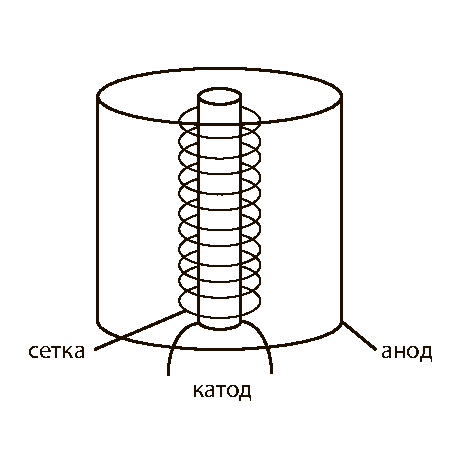
\includegraphics[width=.4\textwidth]{1_1} \hspace{2em}
  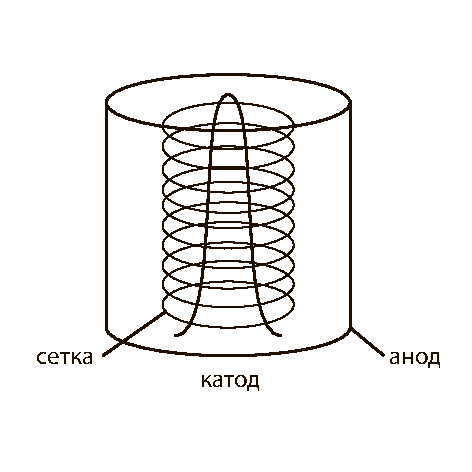
\includegraphics[width=.4\textwidth]{1_2}
  \caption{Конструкция электродов триода}
  \label{pic1}
\end{figure}

Действие управляющей сетки заключается в том, что она регулирует распределение
пространственного заряда между катодом и анодом и, таким образом, управляет
потоком электронов внутри лампы, то есть анодным током. Вследствие того, что
сетка не является сплошной, она свободно пропускает электроны, летящие к аноду.
С другой стороны, она формирует структуру поля, причем резко ослабляется
влияние изменения анодного напряжения на поле вблизи катода --- экранирует
катод от анода и ослабляет действие анода на электроны, вылетающие с катода.

Напряжением на сетке или сеточным напряжением называют разность потенциалов
между сеткой и катодом, то есть потенциал сетки относительно катода. В лампах
с катодом прямого накала все напряжения отсчитывают относительного
отрицательного конца катода.

На рисунке \ref{pic2} показано распределение поля в триоде при различных
величинах напряжения на сетке и фиксированном анодном напряжении. Видно, что
сетка задерживает большую часть поля. Чем гуще сетка, тем сильнее экранирует
она катод от влияния анода. Вследствие этого и отчасти потому, что сетка
расположена ближе к катоду, чем к аноду, небольшие изменения потенциала на
сетке оказывают гораздо более сильное действие на анодный ток, чем значительные
изменения потенциала на аноде.

\begin{figure}[h!]
  \center
  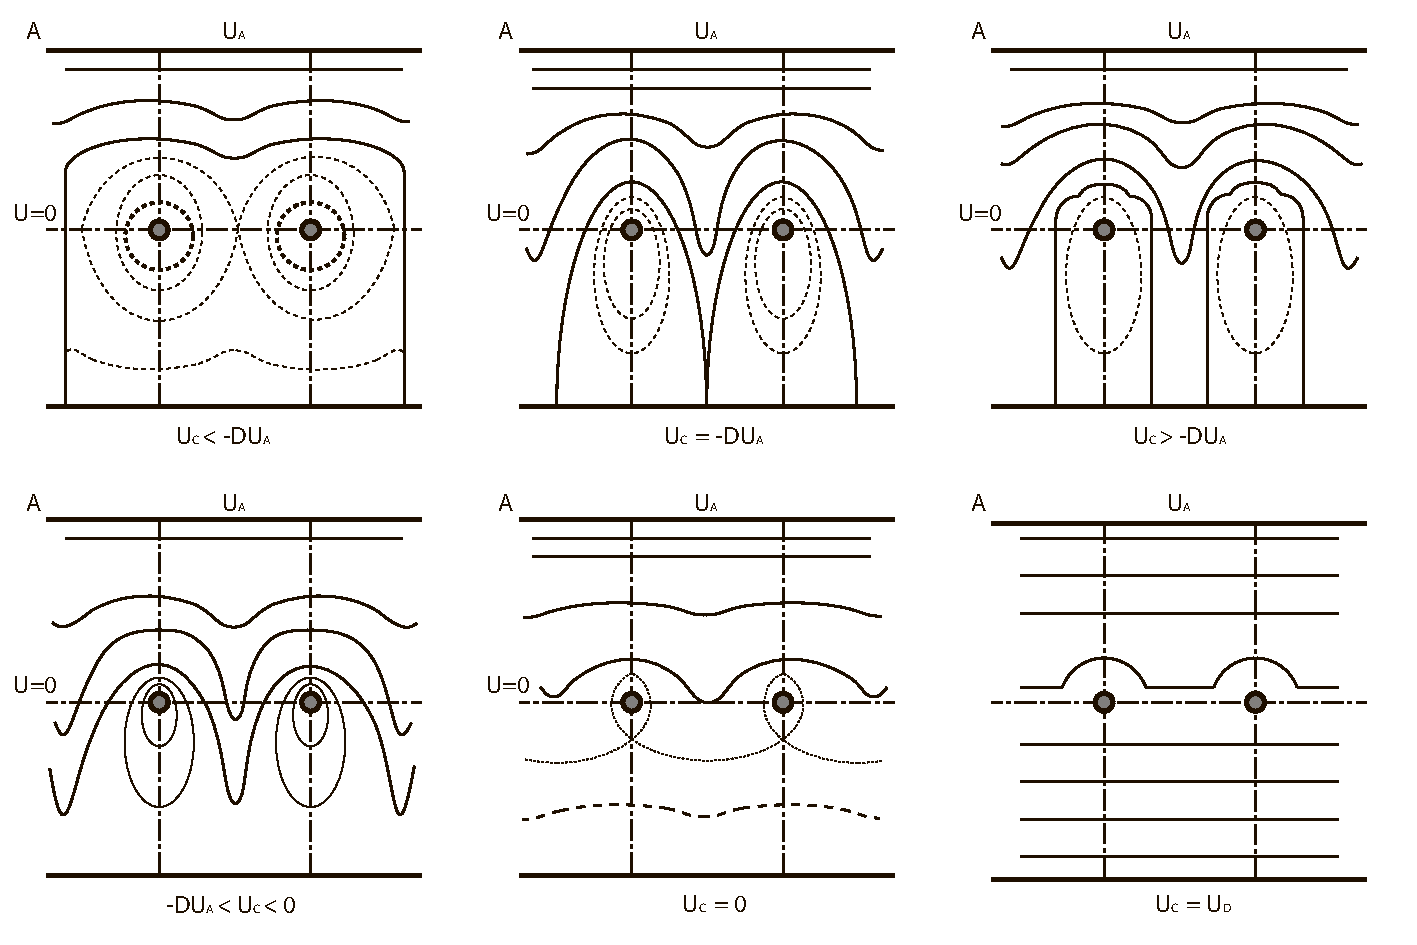
\includegraphics[width=.9\textwidth]{2}
  \caption{Распределение электростатического потенциала плоского триода при
  различных потенциалах сетки и одинаковом анодном напряжении}
  \label{pic2}
\end{figure}

При небольшом отрицательном напряжении сетка отталкивает электроны, но часть их
все же пролетает в ее просветы благодаря притяжению анода. Однако можно
увеличить отрицательное напряжение настолько, что она будет отталкивать все
электроны и анодный ток прекратится. Лампа будет заперта.

\subsubsection{Электродинамика плоского триода}

Для того, чтобы найти распределение потенциала в плоском триоде, найдем
распределение потенциала в системе \( W_1 \), показанной на рисунке~\pic{W1}.

\begin{figure}[h!]
  \center
  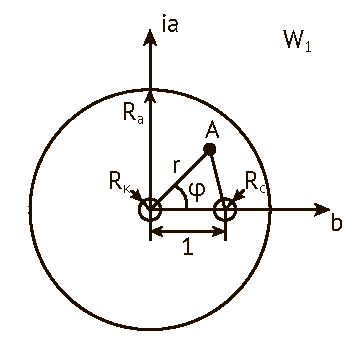
\includegraphics[width=.4\textwidth]{W1} \hspace{1em}
  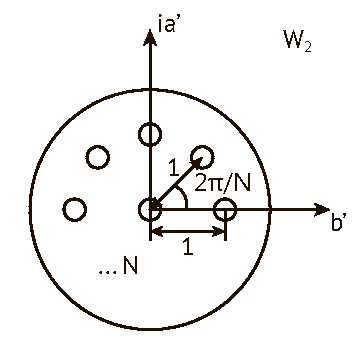
\includegraphics[width=.4\textwidth]{W2} \\
  \parbox{.4\textwidth}{\caption{Комплексная плоскость \( W_1 \)}
    \label{picW1}} \hspace{1em}
  \parbox{.4\textwidth}{\caption{Комплексная плоскость \( W_2 \)}
    \label{picW2}}
\end{figure}

\( W_1 \) состоит из трех цилиндрических электродов: катода, несущего заряд
\( q_k \) и радиусом \( R_k \), элемента сетки, несущего \( q_c \) и радиусом
\( q_c \), и анода, радиусом \( R_a \). Между сеткой и катодом расстояние
принято за единицу. Радиусы сетки и катода значительно меньше расстояний между
сеткой и катодом и сеткой и анодом.

В точке \( A \) наводится следующий потенциал:
\begin{equation}
  U(r, \phi) = \frac{1}{2\pi\Ez}\left[ q_k \ln r + q_c\ln\sqrt{r^2 + 1 -
    2r\cos\phi} \right] + B.
  \label{eqU1}
\end{equation}

Преобразуем комплексную плоскость по закону \( W_2 = (W_1)^{1 / N} =
(re^{i\phi})^{1 / N} \), где \( N \)~-- некоторое число; получим систему
\( W_2 \), изображенную на рисунке~\pic{W2}.

Вместо одного элемента сетки в преобразованной системе будет \( N \) элементов,
отстоящих друг от друга на угол \( 2\pi / N \) и удаленных от катода на
расстояние, равном единице.

Преобразуем комплексную плоскость \( W_2 \) по закону
\[
  W = \ln(W_2) = \ln\left[ (re^{i\phi})^{1 / N} \right] = \frac{1}{N}\ln r +
    i\phi / N = x + iy.
\]

Получим плоскость, изображенную на рисунке~\pic{W}. В плоскости \( x = 0 \)
лежит сетка, в плоскости \( x = -d_\text{кс} = \ln\left[ R_k^{1 / N}
\right] \)~-- катод, в плоскости \( x = d_\text{са} =
\ln\left[ R_a^{1 / N} \right] \)~-- анод.

\begin{figure}[ht!]
  \center
  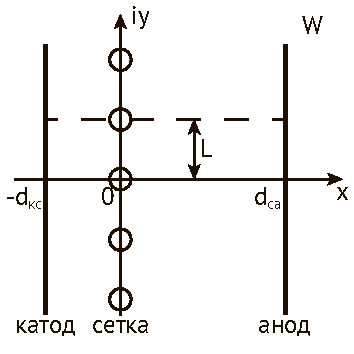
\includegraphics[width=.45\textwidth]{W} \\
  \caption{Комплексная плоскость \( W \)}
  \label{picW}
\end{figure}

Из закона преобразования найдем связь между координатами \( x, y \) и
\( r, \phi \):
\[
  x = \frac{1}{N}\ln r, \quad y = \phi / N; \qquad
    r = e^{xN}, \quad \phi = yN.
\]

Используя последнее соотношение, выразим число \( N \) через расстояние между
элементами сетки \( L \): \( 2\pi = LN \), откуда \( N = 2\pi / L \). Тогда:
\[
  r = \exp\left( \frac{2\pi}{L}x \right), \quad
  \phi = \frac{2\pi}{L}y.
\]

Подставим это в \eqref{eqU1}:
\[
  U(x, y) = \frac{1}{2\pi\Ez} \left[ q_k\frac{2\pi}{L}x + q_c \ln
    \sqrt{e^{4\pi x / L} + 1 - 2e^{2\pi x / L}\cos\frac{2\pi}{L}y} \right] + B.
\]

Граничные условия:
\begin{align*}
  & U(-d_\text{кс},\ y) = 0, \\
  & U(0,\ R_C) = U_C, \\
  & U(d_\text{са},\ y) = U_A,
\end{align*}
где \( R_C = \ln\left[ R_c^{1 / N} \right] \).

Из первого условия найдем константу \( B \).
\[
  0 = \frac{1}{2\pi\Ez} \left[ -q_k\frac{2\pi}{L}d_\text{кс} + \frac{q_c}{2}\ln
    \left( e^{-4\pi d_\text{кс} / L} + 1 - 2e^{-2\pi d_\text{кс} / L}
    \cos\frac{2\pi}{L}y \right) \right] + B.
\]

Так как \( L \ll d_\text{кс} \), то экспонентами относительно единицы можем
пренебречь, и тогда:
\[
  B = \frac{q_k d_\text{кс}}{L\Ez}.
\]

Таком образом,
\begin{equation}
  U(x, y) = \frac{1}{2\pi\Ez} \left[ q_k\frac{2\pi}{L}(x + d_\text{кс}) +
    \frac{q_c}{2} \ln\left( e^{4\pi x / L} + 1 - 2e^{2\pi x / L}
    \cos\frac{2\pi}{L}y \right) \right].
  \label{eqU}
\end{equation}

Из второго условия найдем \( U_C \):
\begin{equation}
  U_C = \frac{1}{2\pi\Ez} \left[ q_k\frac{2\pi}{L}d_\text{кс} + q_c
    \ln\left( 2\sin\frac{pi}{L}R_C \right) \right].
  \label{eqUC}
\end{equation}

Из третьего~-- \( U_A \), учитывая, что \( d_\text{са} \gg\gg L \):
\begin{equation}
  U_A = \frac{1}{2\pi\Ez} \left[ q_k\frac{2\pi}{L}\d_\text{ка} + q_c
    \frac{2\pi}{L}d_\text{са} \right],
  \label{eqUA}
\end{equation}
где \( d_\text{са} = d_\text{кс} + d_\text{са} \)~-- расстояние от катода до
анода.

Решая систему из уравнений \eqref{eqUC} и \eqref{eqUA} относительно неизвестных
зарядов \( q_k \) и \( q_c \) и подставляя их в \eqref{eqU}, получим:
\begin{gather*}
  U(x, y) = \frac{\left\{ -U_A \dfrac{L}{2\pi} \ln\left[ 2\sin\left(
    \dfrac{\pi R_C}{L} \right) \right] + U_C d_\text{са} \right\} \cdot
    \Big( x + d_\text{кс} \Big)}{\left\{ d_\text{ас} d_\text{кс} - d_\text{ка}
    \dfrac{L}{2\pi} \ln\left[ 2\sin\left( \dfrac{\pi R_C}{L}
    \right) \right] \right\}} + \\
  + \frac{\dfrac{L}{4\pi} \ln\left[ 1 + \exp\left( \dfrac{4\pi x}{L} \right) -
    2\exp\left( \dfrac{2\pi x}{L} \right) \cos\left( \dfrac{2\pi y}{L} \right)
    \right] \cdot \Big(U_A d_\text{кс} - U_C d_\text{ка} \Big)}{\left\{
    d_\text{ас} d_\text{кс} - d_\text{ка} \dfrac{L}{2\pi} \ln\left[
    2\sin\left( \dfrac{\pi R_C}{L} \right) \right] \right\}}.
\end{gather*}

Усредним данный потенциал в плоскости сетки \( U(0, y) \) в пределах между
элементами, учитывая, что \( L \ll d_\text{са}, d_\text{ск}, d_\text{ка} \).
Данный потенциал будет называться действующим. Его можно свести к виду
\begin{equation}
  U_D = \sigma (U_C + D U_A),
  \label{eqUD}
\end{equation}
где коэффициент
\[
  D = \frac{1}{\pi d_\text{са}} \int\limits_{R_C}^{L / 2} \ln\left[
    \frac{\sin\left( \dfrac{\pi y}{L} \right)}{\sin\left( \dfrac{\pi R_C}{L}
    \right)} \right]
\]
носит название проницаемости сетки, а \( \sigma \)~-- острота управления:
\[
  \sigma = 1 + \left( \frac{1}{d_\text{ас}} + \frac{1}{d_\text{ск}} \right)
    \frac{L}{2\pi} \ln\frac{L}{2\pi R_C}.
\]

\subsubsection{Эквивалентный диод}

В общем случае анализ электроники триода основан на формуле~\eqref{eqUD}.

Тогда, если предположить, что все электроны, пересекающие область сетки,
достигают анода, прохождение тока можно описать, введя представление
эквивалентного диода, то есть такого диода, у которого плоскость анода
совпадает с плоскостью сетки в триоде. В этом случае катодный ток подчиняется
классическому закону Ленгмюра:
\begin{equation}
  I_k = P(U_C + DU_A)^{3/2}.
  \label{eq1}
\end{equation}

В этом случае условие прекращение анодного тока соответствует равенству
\begin{equation}
  U_C = -DU_A.
  \label{eq2}
\end{equation}

При увеличении напряжения на сетке (но при условии, что \( U_C < 0 \)) анодный
ток совпадает по величине с катодным и растет по закону Ленгмюра \eqref{eq1}.

В результате характер изменения анодного тока в триоде может быть описан двумя
характеристиками: анодно-сеточной, когда при фиксированном анодном напряжении
изменяется напряжение на сетке (рис.~\ref{pic3}), и анодной, когда
напряжение на сетке остается постоянным, но варьируется величина напряжения на
аноде (рис.~\ref{pic4}). Обе характеристики взаимосвязаны~--- и по семейству
анодно-сеточных характеристик легко построить анодную.

\begin{figure}[t!]
  \center
  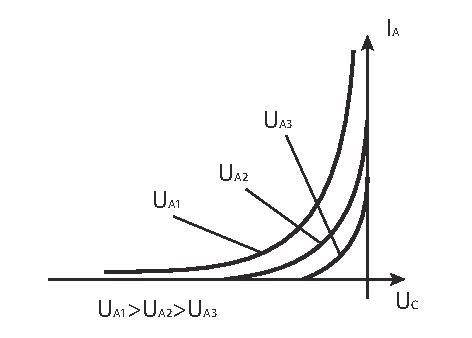
\includegraphics[width=.45\textwidth]{3} \hspace{2em}
  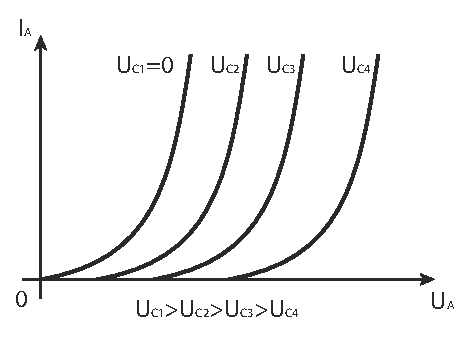
\includegraphics[width=.45\textwidth]{4}
  \parbox{.45\textwidth}{\caption{Семейство анодно-сеточных характеристик
  триода}\label{pic3}} \hspace{2em}
  \parbox{.45\textwidth}{\caption{Семейство анодных характеристик триода}
  \label{pic4}}
\end{figure}

Однако при положительных напряжениях на сетке картина существенно изменяется.
Когда \( U_A > U_D \), все электроны, пролетевшие плоскость сетки, попадают на
анод и сеточный ток определяется лишь теми электронами, которые перехватываются
сеткой при их прямом движении к аноду. Такой режим носит название \emph{режима
токоперехвата}. Он существует до тех пор, пока напряжение на аноде не
сравняется с действующим напряжением. Это означает, что граничный потенциал на
сетке определяется условием \( U_A = U_D \), или
\[
  \left( \frac{U_A}{U_C} \right)_\emph{гр} = \frac{\sigma}{1 - D\sigma}.
\]
Начинается этот режим при положительных напряжениях на сетке.

Введем коэффициент токопрохождения \( s = I_a/I_k \) и коэффициент
токораспределения \( k = I_a/I_c \). Оба эти коэффициента равнозначны, но чаще
используют коэффициент \( s \), зная который легко определяются величины всех
токов:
\[
  I_a = s I_k; \qquad I_c = (1 - s) I_k.
\]

Самая простая оценка величины коэффициента токопрохождения в режиме
токоперехвата может быть сделана при сравнении характера траекторий электронов,
когда напряжение на сетке равно действующему: \( U_C = U_D \), или
\[
  \left( \frac{U_A}{U_C} \right)_1 = \left( \frac{1}{\sigma} - 1 \right)
  \frac{1}{D}; \qquad s = s_1.
\]

В этом случае распределение потенциала в плоском триоде практически совпадает
с распределением потенциала в плоском диоде с расстоянием между анодом и катодом
равном расстоянию между сеткой и катодом. При
\( \left( \cfrac{U_C}{U_D} \right) < 1 \) витки сетки отталкивают электроны,
число электронов, перехватываемых сеткой, уменьшается и \( s \) становится
больше \( s_1 \). При \( \left( \cfrac{U_C}{U_D} \right) > 1 \) витки сетки
начинают играть роль рассеивающей линзы.

Оценить величину коэффициента токопрохождения можно достаточно просто. В случае
\( s = s_1 \) на сетку будут попадать лишь те электроны, которые вылетают из
катода прямо под сеткой. Тогда, если эмиссия из катода равномерна,
\( s_1 = 1 - \cfrac{2R_C}{L} \). При \( \left( \cfrac{U_C}{U_D} \right) < 1 \)
коэффициент токопрохождения растет, при
\( \left( \cfrac{U_C}{U_D} \right) > 1 \) -- падает, причем изменение \( s \)
связано с изменением эффективного электрического радиуса сетки
\( R_{C\,\text{эфф}} \) -- радиуса, который определяет попадание электрона на
сетку.

\begin{figure}[b!]
  \center
  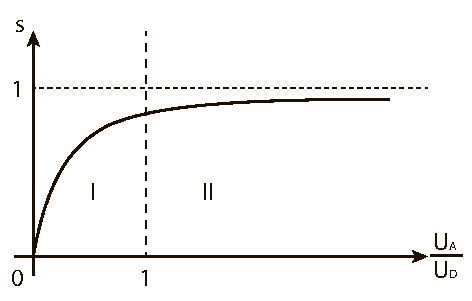
\includegraphics[width=.5\textwidth]{5}
  \caption{Кривая токораспределения в плоском триоде\\
  1 -- область возврата электронов; 2 -- область токоперехвата}
  \label{pic5}
\end{figure}

Когда \( U_D > U_A \), в промежутке между сеткой и анодом на электроны
действует тормозящее поле и не все электроны долетают до анода. Такой режим
носит название \emph{режима возврата электронов}. Ток сетки при этом в основном
определяется теми электронами, которые возвращаются от анода к сетке.

На рисунке \ref{pic5} приведены типичные кривые токораспределения (без учета
начальных скоростей электронов и полей пространственного заряда).

\section{Описание экспериментальной установки}

На рисунке~\ref{picLook} приведен внешний вид экспериментальной установки по
изучению статических характеристик триода.

\begin{figure}[ht]
  \center
  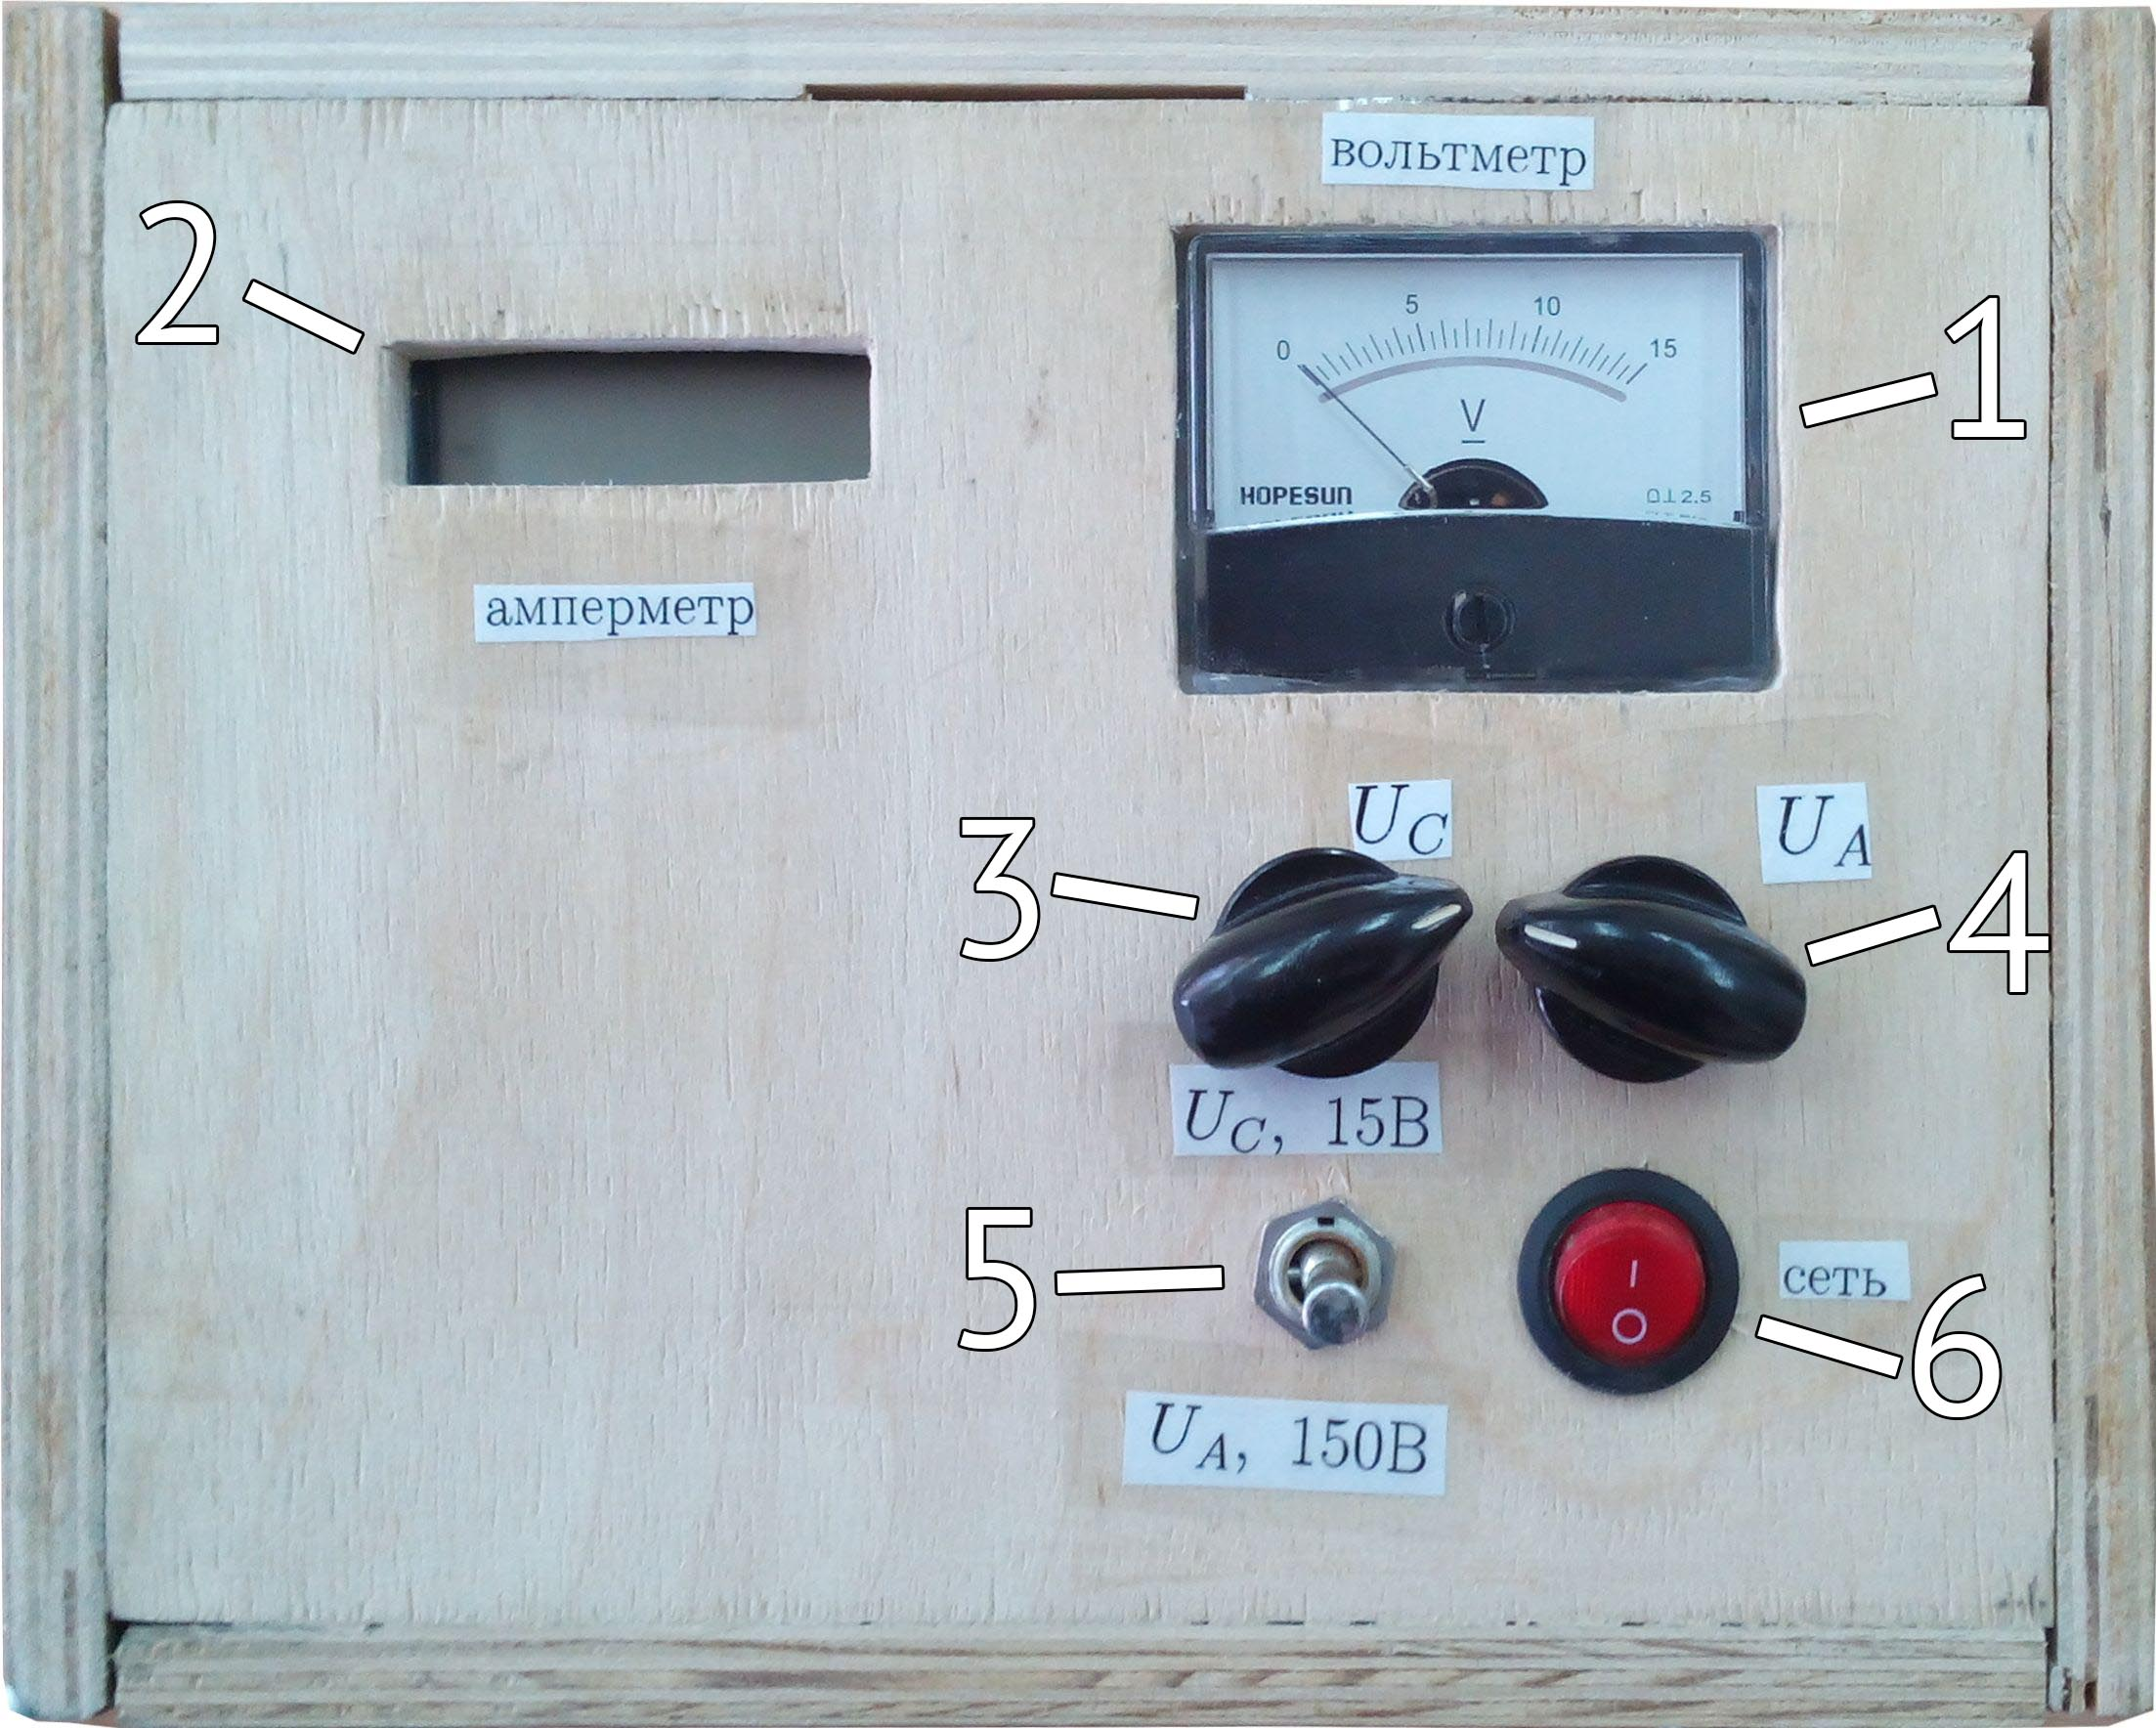
\includegraphics[width=.5\textwidth]{photo}
    \caption{Внешний вид экспериментальной установки} \label{picLook}
\end{figure}

\begin{enumerate}
  \item Вольтметр.
  \item Амперметр.
  \item Регулятор сеточного напряжения.
  \item Регулятор анодного напряжения.
  \item Переключатель измеряемого напряжения.
  \item Выключатель сетевого напряжения.
\end{enumerate}

\begin{figure}[ht]
  \center
  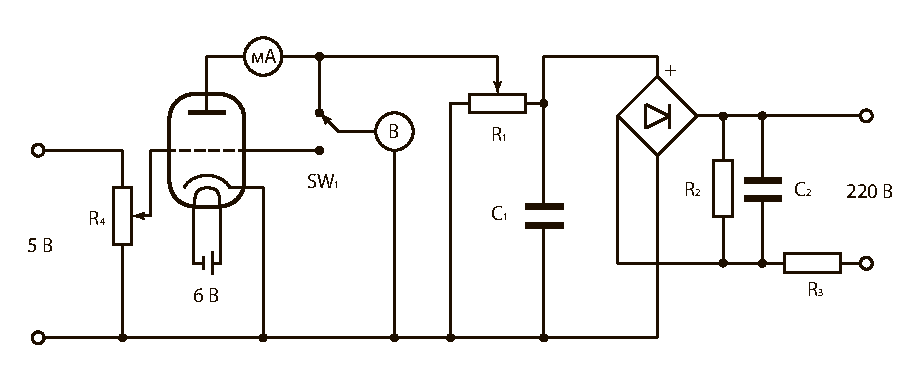
\includegraphics[width=.8\textwidth]{scheme}
    \caption{Принципиальная электрическая схема установки} \label{picScheme}
\end{figure}

Принципиальная схема экспериментальной установки представлена на
рисунке~\ref{picScheme}.

\section{Методика проведения эксперимента}
\renewcommand{\labelenumi}{4.\arabic{enumi}.}
\begin{enumerate}
  \item Включив сеть, дать прибору прогреться не менее 3~мин.
  
  \item Переключатель~5 должен находиться в положении <<\( U_A \)>>, а
    регулятор~3 должен быть повернут вправо до упора.
    \begin{table}[b!]
      \center
      \caption{Семейство анодно-сеточных характеристик}
      \label{grid-anod}
      \begin{tabular}{|m{.1\textwidth}|C{.1}|*{7}{C{.07}|}} \hline
        \multirow{5}{*}{\( U_{a_{01}} \)} &
          \( U_c \),~В &&&&&&& \\ \cline{2-9}
        & \( I_{a_1} \),~мА &&&&&&& \\ \cline{2-9}
        & \( I_{a_2} \),~мА &&&&&&& \\ \cline{2-9}
        & \( I_{a_3} \),~мА &&&&&&& \\ \cline{2-9}
        & \( \average{I_a} \),~мА &&&&&&& \\ \hline
        \multirow{4}{*}{\( U_{a_{02}} \)} &
          \( U_c \),~В &&&&&&& \\ \cline{2-9}
        \multirow{4}{*}{и т.~д.} &
          \( I_{a_1} \),~мА &&&&&&& \\ \cline{2-9}
        & \( I_{a_2} \),~мА &&&&&&& \\ \cline{2-9}
        & \( I_{a_3} \),~мА &&&&&&& \\ \cline{2-9}
        & \( \average{I_a} \),~мА &&&&&&& \\ \hline
      \end{tabular}
    \end{table}

  \item Подать на анод максимально возможное напряжение регулятором~4\\
    (\( U_{a_m} \sim \)40~В). Зафиксировать значение анодного тока.
    
  \item Переключив тумблер~5 в положение <<\( U_C \)>>, повысить по модулю
    напряжение на сетке на одно деление регулятором~3. Переключить~5 в положение
    <<\( U_A \)>> и регулятором~4 вернуть напряжение на аноде к \( U_{a_m} \).
    Записать значение анодного тока.
    
  \item Повторяя пункт~4 для различных \( U_{a_m} \), снять зависимость
    \( I_a(U_c) \) при \( U_a = \const \). Данные занести в
    таблицу~\ref{grid-anod}.

  \item Зафиксировав напряжение на сетке регулятором~3, изменять напряжение на
    аноде регулятором~4 и снять зависимость \( I_a(U_a) \) при
    \( U_c = \const \).

  \item Повторить пункт~6 для различных напряжениях на сетке \( U_c = \const \).
    Результаты занести в таблицу~\ref{anod-anod}.
    
    \begin{table}[ht]
      \center
      \caption{Семейство анодных характеристик триода}
      \label{anod-anod}
      \begin{tabular}{|m{.1\textwidth}|C{.1}|*{7}{C{.07}|}} \hline
        \multirow{5}{*}{\( U_{c_{01}} \)} &
          \( U_a \),~В &&&&&&& \\ \cline{2-9}
        & \( I_{a_1} \),~мА &&&&&&& \\ \cline{2-9}
        & \( I_{a_2} \),~мА &&&&&&& \\ \cline{2-9}
        & \( I_{a_3} \),~мА &&&&&&& \\ \cline{2-9}
        & \( \average{I_a} \),~мА &&&&&&& \\ \hline
        \multirow{4}{*}{\( U_{c_{02}} \)} &
          \( U_a \),~В &&&&&&& \\ \cline{2-9}
        \multirow{4}{*}{и т.~д.} &
          \( I_{a_1} \),~мА &&&&&&& \\ \cline{2-9}
        & \( I_{a_2} \),~мА &&&&&&& \\ \cline{2-9}
        & \( I_{a_3} \),~мА &&&&&&& \\ \cline{2-9}
        & \( \average{I_a} \),~мА &&&&&&& \\ \hline
      \end{tabular}
    \end{table}
    
    \item Построить графики анодно-сеточной и анодной характеристик на
      миллиметровой бумаге.

    \item По экспериментально определенным анодно-сеточным характеристикам
      построить семейство анодных характеристик и сравнить с анодными
      характеристиками, полученными экспериментально.
\end{enumerate}

\end{document}
